%% Template for a preprint Letter or Article for submission
%% to the journal Nature.
%% Written by Peter Czoschke, 26 February 2004
%%


\documentclass{nature}

%\usepackage[backend=biber]{biblatex}
\usepackage{graphicx}
%% make sure you have the nature.cls and naturemag.bst files where
%% LaTeX can find them

%\bibliographystyle{naturemag}

\title{The Missing Baryon Problem: Investigating missing matter using the Universe's first picture}

%% Notice placement of commas and superscripts and use of &
%% in the author list

\author{Mitchell de Zylva$^{1}$}


\begin{document}

\maketitle

\begin{affiliations}
 \item The University of Melbourne, Victoria, Australia
\end{affiliations}

%\begin{abstract}

\begin{figure}
    \begin{center}
        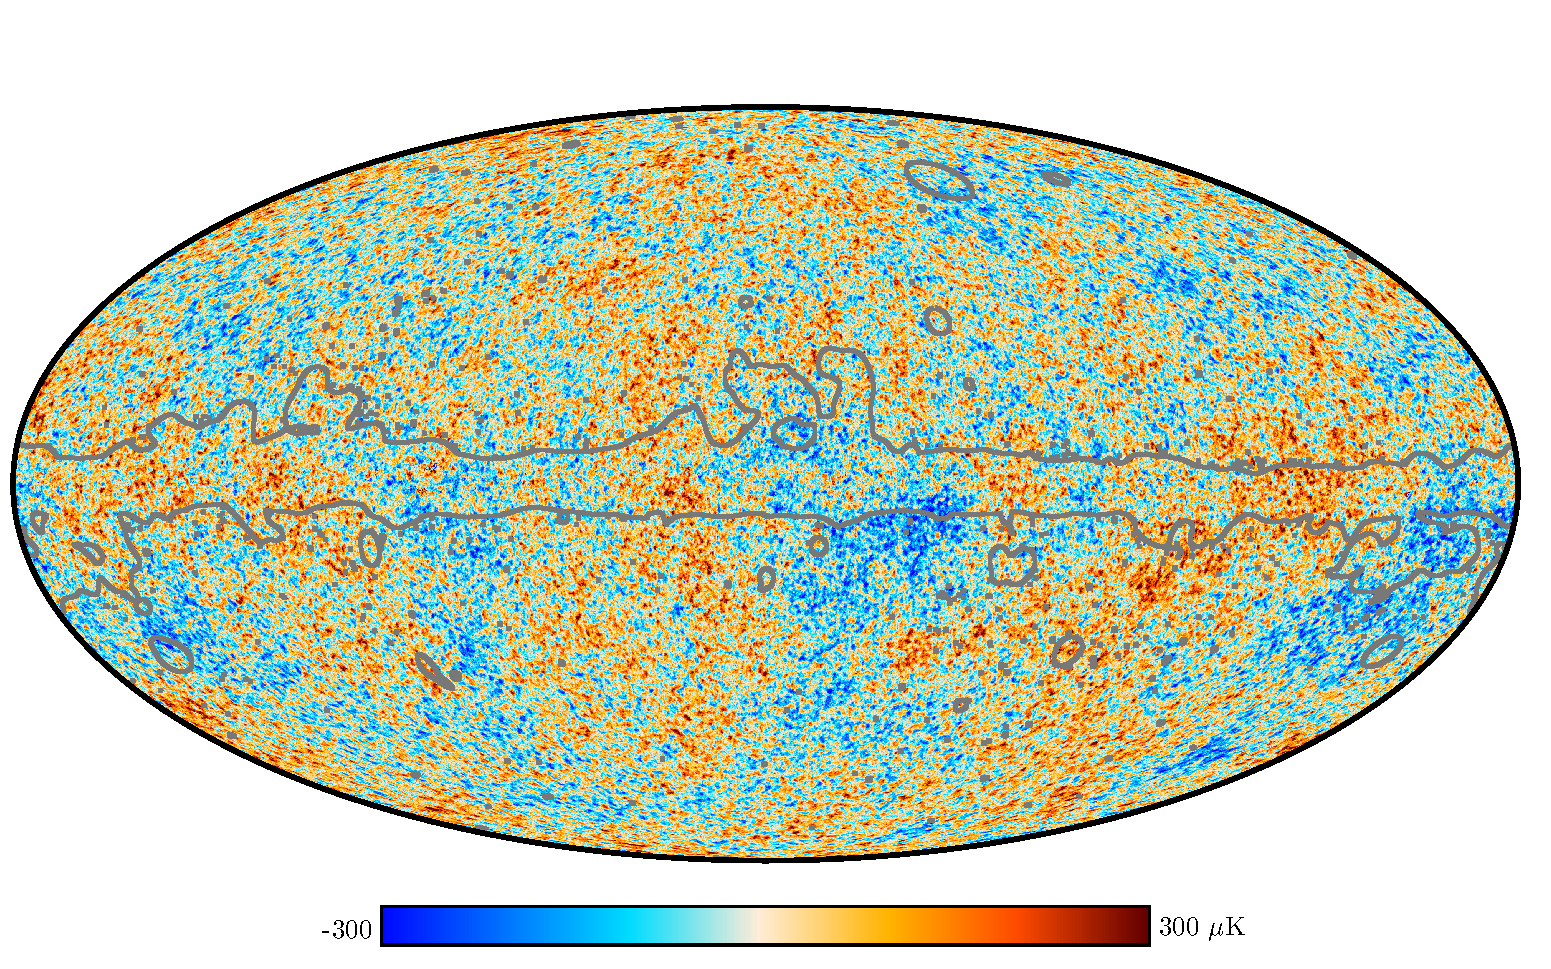
\includegraphics[scale=0.5]{Planck_2018_T_CMB.pdf}
        \caption{This is a figure.}
    \end{center}
\end{figure}

Fifty five years after its accidental discovery, the first image of a baby universe has still not given up all its secrets. The afterglow of the Big Bang, known as the Cosmic Microwave Background (CMB), is the only faint remnant of the early universe currently still visible in the sky, and it has been central in ushering in a golden age of cosmology.  
%\end{abstract}

The CMB is made up of very low power microwaves, and its characteristic splotches provide key insights into conditions in the early universe, allow astronomers to determine characteristics, such as the relative proportions of matter, dark matter and dark energy, and other fundamental parameters. To date, they yield the most precise measures of the age, geometry and composition of the universe we have. 

In more recent years, a number of experiments have been done specifically to examine the properties of the CMB, including the Atacama Cosmology Telescope in the mountains of Chile, the South Pole Telescope, and the European Space Agency's \textit{Planck} Satellite. These experiments have broadened the scope of the original detection, leading to the collection of an unprecedented amount of data, and applications across a number of areas of astronomy. 

\section{The Missing Baryon Problem}
The CMB has allowed us to determine with a very high level of confidence the composition of the universe. The universe is broadly comprised of light, regular matter, and the infamous dark matter and dark energy, and the precise ratios of each are very tightly constrained. 

However when astronomers look at the sky, and measure the amount of matter they see with telescopes, it becomes apparent that only about half of the universe's regular matter - known as 'baryons' - is present in the light emitted from stars and galaxies. This begged the question, where was all the missing matter? 

It was clear that the matter must be there, since it is very clear to discern between dark matter and baryons in physical models. The universe could not have evolved to be what we see today if that fraction wasn't correct. But it was also apparent that only about 10 percent of baeyons exist in galaxies themselves, with some 30 to 40 percent existing in gas clouds surrounding galaxies. This still leaves a large fraction unaccounted for. 

A possible answer comes from simulations. When astronomers model the behaviour of the very early universe, they notice that when galaxies form, long string like filaments form between them, creating a picture not unlike those seen in the brain with neurons.
They call these filaments the Warm-Hot Intergalactic Medium, or "WHIM". 
\begin{figure}
    \includegraphics{tiamat_1.png}
\end{figure}


These filaments contain very small amounts of matter, superheated to temperatures between thousands and millions of degrees, and spread out over the vast reaches of space. The combination of its speed and the distances over which it is spread makes thes filaments very sparse - only a few atoms per cubic meter. 

Detecting these filaments has proven to be a difficult task, since the scarcity of the gas makes it very unlikely that there will be any observable signal. The only possible method of direct detection of this matter involves using a quasar, a galaxy with a very active super-massive black hole at its centre, as a backlight. Unfortunately this is an incredibly rare event, since it requires us to find just such an object, and for its beam to pass through both a filament and a telescope that is observing the sky and can see the object. 

Citation of Einstein's paper \cite{Einstein}.

\bibliographystyle{naturemag}
\bibliography{sample}
\end{document}
Citation of Einstein's paper \cite{Einstein}.
